\chapter{Theoretical Background}\label{chapter:background}

{ \color{red}

    about 20-30 pages (rather less I guess?)

    \begin{enumerate}
        \item Introduction to XAI in general
        \item Evaluation of XAI methods in general
        \item Structural Causal Models and causal framework
    \end{enumerate}
}

\section{Neural Networks}
\todo{General explanation of neural networks}
\begin{itemize}
    \item Explain all general concepts that are needed for understanding CRP etc. 
    \item neurons and layers
    \item convolutional layers and channels
    \item linear layers and output layer
    \item activation functions (especially ReLU)
    \item MaxPooling layer 
    \item backpropagation / forward
    \item optimizers (specifically Adam) - learning rate
    \item loss function (here CrossEntropyLoss)
    \item training? batch size
\end{itemize}

\section{Layerwise Relevance Propagation}
Layer-wise relevance propagation \cite{Bach2015} is the basis for concept relevance propagation and is next to SHAP, LIME, Integrated Gradients \todo{cite} among the most highly cited local attribution methods in XAI. As other saliency methods, LRP is commonly used in computer vision tasks to attribute importance to each pixel in an image, which can then be visualized as a heatmap, but is also applicable to other data formats. In the following I will summarize the basic functioning of LRP for neural networks as described in \cite{Bach2015}:

LRP assumes that the model has multiple layers of computation it can be decomposed into, starting from the input layer, for example the pixels of an image, to all latent layers $l$ and finally to the output layer. Further each of those layers has $V(l)$ dimensions for which a Relevance Score $R^{(l)}_d$ could be determined so that the following equation holds:

\begin{equation}
    f(x) = ... = \sum_{d \in l+1} R^{(l+1)}_d =  \sum_{d \in l} R^{(l)}_d = ... =  \sum_{d} R^{(1)}_d
\end{equation}

In neural networks, the general forward step for one layer most often includes weighing the previous layers outputs $x_i$ with the current layers weights $z_{ij} = x_i w_{ij}$, summing the results for all connected neurons and their bias $z_{j} = \sum_{i} z_{ij} + b_j$ and running this through a non-linear activation function $x_j = \sigma (z_j)$.
The idea then is to follow the flow of relevance from the output, where usually the prediction value is taken to initialize the relevance $R^(1)_d$, back to the input layer by decomposition. In the simplest case relevance is proportionally propagated back to the previous layer where the relevance of all connected neurons is aggregated in the following:
\begin{equation}
    R_i = \sum_{j}  R_{i_j} = \sum_{j} \frac{z_{ij}}{z_j} R_j
\end{equation}

To apply LRP, best practices and rules have emerged \cite{Kohlbrenner2020, Montavon2019, Samek2021}. However in this thesis we stick to the propagation rule that the authors of CRP use, namely the composite $LRP_{\epsilon-z+-\flat}$-rule (or "epsilon-plus-flat"), which is recommended by \cite{Kohlbrenner2020} and uses different rules for different parts of the model, further described in the appendix \autoref{appendix:lrprules}.

\todo{mention that it has been getting a mathematical background with Deep Taylor Decomposition  \cite{Montavon2017}}


\section{Concept Relevance Propagation}

LRP aggregates the significance of all latent layers and their neurons into one importance map, where the intermediate layers outputs are merely a side-product of the computation.
Achtibat et. al. propose in their recent work \cite{Achtibat2022} to use those intermediate results to further disentangle the attributions. While in LRP the initialization at the output layer usually takes the value of one class output $y$ w.r.t input $\mathbf{x}$, all other output neurons set to zero, and thereby produces a class-conditional attribution ($R(\mathbf{x}|y)$), a similar thing can be done in latent layers too. Allthough it is yet unclear how to interpret the attribution to these hidden features, the authors of CRP propose to obtain importance scores for them by computing "(multi-)concept-conditional" relevances $R(\mathbf{x}|\theta)$. The variable $\theta$ here describes a set of conditions $c_l$ which in essence \textit{filters} for certain \textit{concepts} i.e. features in potentially mutliple layers by masking out all other features' contributions:

\begin{equation}
    R^{(l-1, l)}_{i_j} (\mathbf{x} | \theta \cup \theta_l) = \frac{z_{ij}}{z_j} \cdot \sum_{c_l \in \theta_l} \delta_{jc_l} \cdot R^{l}_j (\mathbf{x} | \theta )
\end{equation}

$\delta_{jc_l}$ is the Kronecker-Delta selecting the relevance $R^l_j$ of feature $j$ in layer $l$ if that index is in the condition $c_l$, masking out all other features in that layer. If no condition is set for a particular layer, the relevance from that layer is not masked. The authors note that conditions within the same layer compare to logical OR operations and across layers to AND operations. In the following a small example illustrates the process (\autoref{fig:crp_example_condition}):

\todo{mention new paper which is more summarized: \cite{Achtibat2023}}

\begin{figure}[htbp]
    \centering
    \tikzset{%
        neuron/.style={
                circle,
                draw,
                minimum size=8mm
            },
        neuronlabel/.style={
                circle=none,
                draw=none,
                text height=0.7cm,
            },
        edgelabel/.style={
                circle=none,
                draw=none,
                text height=0.8cm,
            },
        conditioned/.style={
                fill=gray
            },
    }
    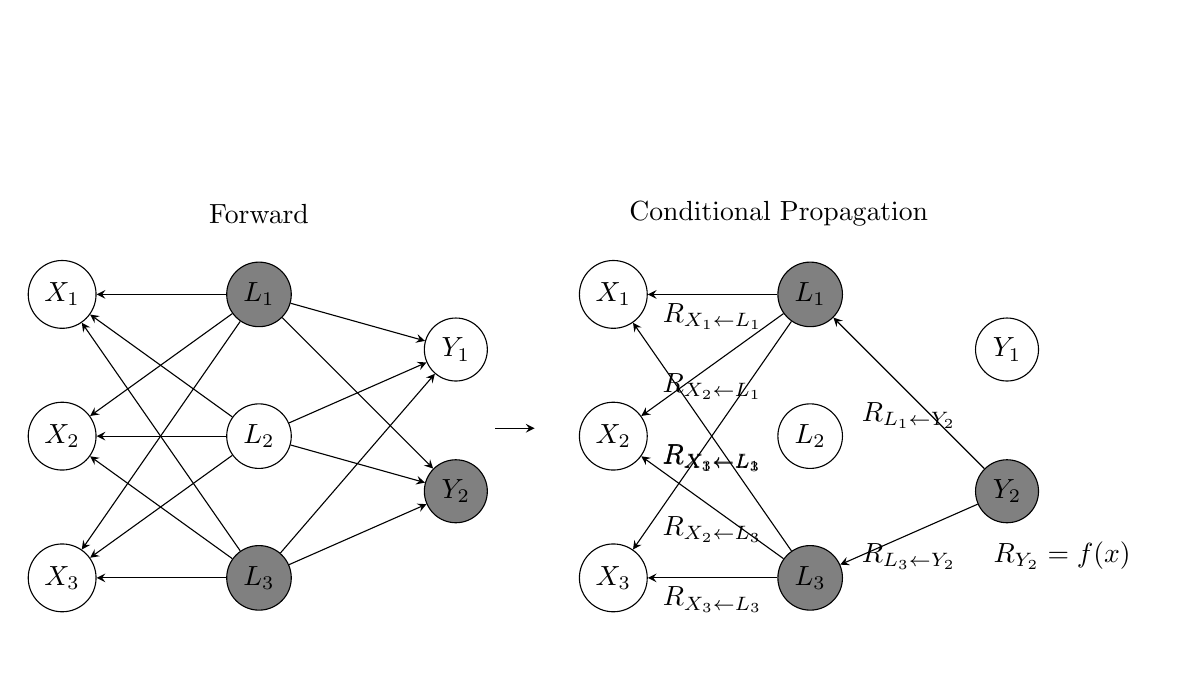
\begin{tikzpicture}[>=stealth,
            every node/.style={ draw, minimum size=8mm, align=center},]

        % First layer
        \foreach \x in {1,2,3} {
                \node [neuron] (X\x) at (0,{-\x* 1.8}) {$X_\x$};
            }
        \node [edgelabel]  (ti1) at (2.5,-0.5) {Forward};
        % Second layer
        \foreach \x in {1,2,3}{
                \pgfmathparse{\x==1 || \x ==3}
                \ifnum \pgfmathresult=1
                    \node  [neuron, conditioned]  (L\x) at (2.5,{-\x* 1.8}) {$L_\x$};
                \else
                    \node  [neuron]  (L\x) at (2.5,{-\x* 1.8}) {$L_\x$};
                \fi
            }

        % Last layer
        \foreach \x in {1,2} {
                \ifnum \x = 2
                    \node [neuron, conditioned]  (Y\x) at (5,{-\x* 1.8 - 0.7}) {$Y_\x$};
                    %\node [neuronlabel] at (Y\x.south) {$R_{Y_\x} = f(x)$};
                \else
                    \node  [neuron]  (Y\x) at (5,{-\x* 1.8 - 0.7}){$Y_\x$};
                \fi
            }

        % Connect nodes
        \foreach \y in {1,2,3}
        \foreach \x in {1,2,3}{
                \ifnum\x=\y
                    \draw[<-] (X\x) -- (L\y);
                    %node[midway, edgelabel] {$R_{X_\x  \gets L\y}$};
                \else
                    \pgfmathparse{2 > \x-\y && 2 > \y-\x}
                    \ifthenelse{\pgfmathresult=1}{\draw[<-] (X\x) -- (L\y);}{}
                \fi
            }
        \foreach \x in {1,2,3}
        \foreach \y in {1,2}
        \draw[->] (L\x) -- (Y\y);

        \draw[->] (5.5,-3.5) -- (6,-3.5);

        % OTHER GRAPH
        % First layer
        \foreach \x in {1,2,3} {
                \node [neuron] (X\x) at (7,{-\x* 1.8}) {$X_\x$};
            }

        % Second layer
        \node [edgelabel]  (ti2) at (9.1,-0.5) {Conditional Propagation};
        \foreach \x in {1,2,3}{
                \pgfmathparse{\x==1 || \x ==3}
                \ifnum \pgfmathresult=1
                    \node  [neuron, conditioned]  (L\x) at (9.5,{-\x* 1.8}) {$L_\x$};
                \else
                    \node  [neuron]  (L\x) at (9.5,{-\x* 1.8}) {$L_\x$};
                \fi
            }

        % Last layer
        \foreach \x in {1,2} {
                \ifnum \x = 2
                    \node [neuron, conditioned]  (Y\x) at (12,{-\x* 1.8 - 0.7}) {$Y_\x$};
                    \node [neuronlabel] at (12.7,{-\x* 1.8 - 1.3}) {$R_{Y_\x} = f(x)$};
                \else
                    \node  [neuron]  (Y\x) at (12,{-\x* 1.8 - 0.7}){$Y_\x$};
                \fi
            }

        % Connect nodes
        \foreach \y in {1,3}
        \foreach \x in {1,2,3}{
                \pgfmathparse{2 > \x-\y && 2 > \y-\x}
                \ifthenelse{\pgfmathresult=1}{\draw[<-] (X\x) -- (L\y)  node[midway, edgelabel] {$R_{X_\x  \gets L_\y}$};}{}
            }
        \foreach \x in {1,3}
        \foreach \y in {2}
        \draw[<-] (L\x) -- (Y\y) node[midway,align=center, edgelabel] {$R_{L_\x  \gets Y_\y}$};
    \end{tikzpicture}

    \caption{Left side: simple neural network forward pass with input layer X, one hidden layer L and output layer Y. Conditioning set $\theta = \{L_1, L_3, Y_2\}$ \\ Right side: only the relevance of the neurons matching the conditioning set is propagated back \\
        Result at input pixel $R_{X_2} = \sum_{j}  R_{X_2 \gets L_j} =  \sum_i \sum_{j} \cdot \frac{a_i w_{ij}}{\sum_h a_h w_{hj}} R_j \dots$ }
    \label{fig:crp_example_condition}
\end{figure}

\subsubsection*{Usage Scenarios}
Heatmaps produced by conditional attribution could be analyzed in a similar fashion to the tradional class-specific heatmaps produced by LRP. The hinderance is that the meanings of the conditioned on latent features are not known, so it is unclear how to interpret the importance of some pixels for feature $i$ in layer $l$. For large, complex models some human-understandable concepts can emerge in hidden layers from simpler more local concepts in earlier and more abstract concepts in later layers \cite{Bau2017, Hohman2020, Olah2017, Bau2020}. However this is not a fact to rely on and seems to regularly fail for smaller models or simpler problems as noted before (\autoref{subsection:evaluation_critique}) and in other work \todo{cite}.

CRP's authors therefore construct a framework for the understanding of these latent features. \textit{Activation Maximization} is used to find the samples for which the neuron (set) of a concept has the highest activation. They build on the idea of activation maximization when proposing \textit{Relevance Maximization}, where samples maximize the conditional relevance of a concept instead of the activation. Both methods yield a set of images or samples (see \autoref{fig:act_rel_max}), which can be enhanced further by masking out the irrelevant parts of the image, creating class specific reference samples and carefully selecting or extending the pool of samples to choose from. 

\begin{figure}[htbp]
    \centering
	\includegraphics[width=0.3\textwidth]{pics/test.png}
    \caption{Activation Maximization in Comparison to Relevance Maximization. The image is cropped to the region with highest activation/relevance thresholded by X. }
    \label{fig:act_rel_max}
\end{figure}
\todo{image of ActMax and RelMax examples (using my dataset?)}

The resulting interpretation tools for single concepts are combined with methods for a local explanation, i.e. the analysis of a single sample or image. A \textit{Concept Atlas} (\autoref{fig:concept_atlas}) inspired by Carter et. al.'s \textit{Activation Atlas} \todo{cite} colors parts of an image based on the most relevant concept in that region. \textit{Hierarchical attribution graphs} (\autoref{fig:attr_graph}) decompose the relevant concepts for an image into their lower layer subconcept channels. The presumption being that the spread of relevance into lower level features helps in the understanding of relevant concepts for a sample.

\begin{figure}[htbp]
    \centering
	\includegraphics[width=0.3\textwidth]{pics/test.png}
    \caption{Concept Atlas}
    \label{fig:concept_atlas}
\end{figure}

\begin{figure}[htbp]
    \centering
	\includegraphics[width=0.3\textwidth]{pics/test.png}
    \caption{Hierarchical attribution graph}
    \label{fig:attr_graph}
\end{figure}
\todo{image of Concept Atlas and hierarchical concept composition}

From these local explanations ... 
first experiments for a more global explanation

\todo{global: Assessing Concept Similarity in Latent Space}

\todo{papers with crp and more global explanation / concept clustering stuff}
other papers (vielhaben, lapuschkin...) do more in this direction
summarize work that builds on top of original CRP paper ?
what else CRP could potentially be used for
\cite{Dreyer2023,Pahde2023,Dreyer2023a,Vielhaben2022,Vielhaben2023,Achtibat2023}

\section{Causal Framework}
\subsection{Structural Causal Models}

\begin{itemize}
    \item Explain and define in detail Structural Causal Models
    \item neural networks could be seen as SCMs \cite{Chattopadhyay2019}
    \item but AI / neural networks in general do not care about causation and work through finding useful correlations
    \item and that is good this way, otherwise they would never find anything useful, statistics and correlations are great
    \item none-the-less the better we get at identifying spurious features the more causal methods might apply?
    \item it doesn't matter whether the network has found the actual causal reasons for its prediction, but explanations are a distinctively causal concept.
    \item and explanation asks how and why, so we want to know the cause of model predicting Y from X
    \item causal methods have started to be used for evaluation of xai
\end{itemize}

\subsection{Interpretation as Interventions}
There is no problem in defining the neural network as a causal model. 
Also, in principle it does not matter which layer we pick out to quantify importance, as the whole importance has to flow through this layer. This is only true for neural network architectures that have no skip-connections or are recurrent and has to be viewed differently in other cases as has already been approached by \cite{Chattopadhyay2019}. However we know, that while the earlier layers of the neural network are more localized and have lower-level features / interpretations, the opposite is true for later layers, encoding more abstract not necessarily localized concepts. 
So when trying to disentangle one features importance from other, one has to find a trade-off between disentanglement and abstraction/conceptual interpretability.
 

\subsection{Data Generation Process}

Other?

\begin{itemize}
    \item Short introduction to causal effects    \item counterfactuals
    \item
\end{itemize}


\section{Evaluation of Explanations}
\subsection{Ground Truth Importance}
\begin{itemize}
    \item What are currently used ground truth importance measures for concepts or latent factors
    \item introduce Prediction Flip with formula or application to our use case
    \item R2 score with formula \cite{Sixt2020}
    \item mean logit change with formula
    \item make clear: human understanding is the ultimate goal, so user studies are the gold standard (but often not well done) but not feasible here
    \item relate to constant vector shift problem and how this might be measured
\end{itemize}
\subsection{CRP Concept Importance Measures}
\todo{need proper measure}
\begin{itemize}
    \item explain the measures i use to score how well the concepts are separated
    \item show theoretical basis
\end{itemize}

\subsubsection*{NOCHMAL: MÖGLICHE DR/CONCEPT ALGORITHMEN:}
\todo{decide on measures to try out / officially add to comparison}
\begin{itemize}
    \item KNN auf allen layers / einer bestimmten layer - relevances mit 4 clustern
    \item NMF auf clamped relevances
    \item "causal effect" von latent factors auf relevanzen
    \item image perturbation - oana
    \item Intersection over union "Weakly supervised location (WSL)" Real Time Image Saliency for Black Box Classifiers
    \item Precision: how many of the important pixels are within the actual object
    \item Earth Movers Distance: cost of trnsforming importance map into F+ (image?) using euclidean distance between pixels
    \item TCAV: user defined concept (e.g. choose only images with watermark) 
    \item Causal Concept Effect (CaCE) (can avoid confounding errors) 
    \item encoder-decoder: try to learn latent factors 
\end{itemize}


\subsection{Causally somehow? }